\documentclass[twoside]{book}

% Packages required by doxygen
\usepackage{fixltx2e}
\usepackage{calc}
\usepackage{doxygen}
\usepackage[export]{adjustbox} % also loads graphicx
\usepackage{graphicx}
\usepackage[utf8]{inputenc}
\usepackage{makeidx}
\usepackage{multicol}
\usepackage{multirow}
\PassOptionsToPackage{warn}{textcomp}
\usepackage{textcomp}
\usepackage[nointegrals]{wasysym}
\usepackage[table]{xcolor}

% Font selection
\usepackage[T1]{fontenc}
\usepackage[scaled=.90]{helvet}
\usepackage{courier}
\usepackage{amssymb}
\usepackage{sectsty}
\renewcommand{\familydefault}{\sfdefault}
\allsectionsfont{%
  \fontseries{bc}\selectfont%
  \color{darkgray}%
}
\renewcommand{\DoxyLabelFont}{%
  \fontseries{bc}\selectfont%
  \color{darkgray}%
}
\newcommand{\+}{\discretionary{\mbox{\scriptsize$\hookleftarrow$}}{}{}}

% Page & text layout
\usepackage{geometry}
\geometry{%
  a4paper,%
  top=2.5cm,%
  bottom=2.5cm,%
  left=2.5cm,%
  right=2.5cm%
}
\tolerance=750
\hfuzz=15pt
\hbadness=750
\setlength{\emergencystretch}{15pt}
\setlength{\parindent}{0cm}
\setlength{\parskip}{3ex plus 2ex minus 2ex}
\makeatletter
\renewcommand{\paragraph}{%
  \@startsection{paragraph}{4}{0ex}{-1.0ex}{1.0ex}{%
    \normalfont\normalsize\bfseries\SS@parafont%
  }%
}
\renewcommand{\subparagraph}{%
  \@startsection{subparagraph}{5}{0ex}{-1.0ex}{1.0ex}{%
    \normalfont\normalsize\bfseries\SS@subparafont%
  }%
}
\makeatother

% Headers & footers
\usepackage{fancyhdr}
\pagestyle{fancyplain}
\fancyhead[LE]{\fancyplain{}{\bfseries\thepage}}
\fancyhead[CE]{\fancyplain{}{}}
\fancyhead[RE]{\fancyplain{}{\bfseries\leftmark}}
\fancyhead[LO]{\fancyplain{}{\bfseries\rightmark}}
\fancyhead[CO]{\fancyplain{}{}}
\fancyhead[RO]{\fancyplain{}{\bfseries\thepage}}
\fancyfoot[LE]{\fancyplain{}{}}
\fancyfoot[CE]{\fancyplain{}{}}
\fancyfoot[RE]{\fancyplain{}{\bfseries\scriptsize Generated by Doxygen }}
\fancyfoot[LO]{\fancyplain{}{\bfseries\scriptsize Generated by Doxygen }}
\fancyfoot[CO]{\fancyplain{}{}}
\fancyfoot[RO]{\fancyplain{}{}}
\renewcommand{\footrulewidth}{0.4pt}
\renewcommand{\chaptermark}[1]{%
  \markboth{#1}{}%
}
\renewcommand{\sectionmark}[1]{%
  \markright{\thesection\ #1}%
}

% Indices & bibliography
\usepackage{natbib}
\usepackage[titles]{tocloft}
\setcounter{tocdepth}{3}
\setcounter{secnumdepth}{5}
\makeindex

% Hyperlinks (required, but should be loaded last)
\usepackage{ifpdf}
\ifpdf
  \usepackage[pdftex,pagebackref=true]{hyperref}
\else
  \usepackage[ps2pdf,pagebackref=true]{hyperref}
\fi
\hypersetup{%
  colorlinks=true,%
  linkcolor=blue,%
  citecolor=blue,%
  unicode%
}

% Custom commands
\newcommand{\clearemptydoublepage}{%
  \newpage{\pagestyle{empty}\cleardoublepage}%
}

\usepackage{caption}
\captionsetup{labelsep=space,justification=centering,font={bf},singlelinecheck=off,skip=4pt,position=top}

%===== C O N T E N T S =====

\begin{document}

% Titlepage & ToC
\hypersetup{pageanchor=false,
             bookmarksnumbered=true,
             pdfencoding=unicode
            }
\pagenumbering{roman}
\begin{titlepage}
\vspace*{7cm}
\begin{center}%
{\Large My Project }\\
\vspace*{1cm}
{\large Generated by Doxygen 1.8.11}\\
\end{center}
\end{titlepage}
\clearemptydoublepage
\tableofcontents
\clearemptydoublepage
\pagenumbering{arabic}
\hypersetup{pageanchor=true}

%--- Begin generated contents ---
\chapter{Class Index}
\section{Class List}
Here are the classes, structs, unions and interfaces with brief descriptions\+:\begin{DoxyCompactList}
\item\contentsline{section}{\hyperlink{structnode}{node} }{\pageref{structnode}}{}
\item\contentsline{section}{\hyperlink{structnode1}{node1} }{\pageref{structnode1}}{}
\item\contentsline{section}{\hyperlink{structnode__info}{node\+\_\+info} }{\pageref{structnode__info}}{}
\end{DoxyCompactList}

\chapter{File Index}
\section{File List}
Here is a list of all files with brief descriptions\+:\begin{DoxyCompactList}
\item\contentsline{section}{\hyperlink{Lab1_8c}{Lab1.\+c} }{\pageref{Lab1_8c}}{}
\end{DoxyCompactList}

\chapter{Class Documentation}
\hypertarget{structnode}{}\section{node Struct Reference}
\label{structnode}\index{node@{node}}


Collaboration diagram for node\+:
\nopagebreak
\begin{figure}[H]
\begin{center}
\leavevmode
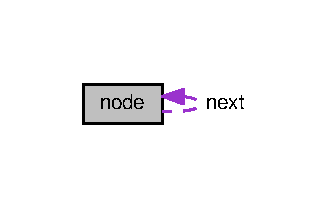
\includegraphics[width=158pt]{structnode__coll__graph}
\end{center}
\end{figure}
\subsection*{Public Attributes}
\begin{DoxyCompactItemize}
\item 
int \hyperlink{structnode_a2d890bb9f6af0ffd73fe79b21124c2a2}{data}
\item 
\hyperlink{structnode}{node} $\ast$ \hyperlink{structnode_aad210fa7c160a49f6b9a3ffee592a2bc}{next}
\end{DoxyCompactItemize}


\subsection{Member Data Documentation}
\index{node@{node}!data@{data}}
\index{data@{data}!node@{node}}
\subsubsection[{\texorpdfstring{data}{data}}]{\setlength{\rightskip}{0pt plus 5cm}int node\+::data}\hypertarget{structnode_a2d890bb9f6af0ffd73fe79b21124c2a2}{}\label{structnode_a2d890bb9f6af0ffd73fe79b21124c2a2}
\index{node@{node}!next@{next}}
\index{next@{next}!node@{node}}
\subsubsection[{\texorpdfstring{next}{next}}]{\setlength{\rightskip}{0pt plus 5cm}{\bf node}$\ast$ node\+::next}\hypertarget{structnode_aad210fa7c160a49f6b9a3ffee592a2bc}{}\label{structnode_aad210fa7c160a49f6b9a3ffee592a2bc}


The documentation for this struct was generated from the following file\+:\begin{DoxyCompactItemize}
\item 
\hyperlink{SelfOrganizing_8cpp}{Self\+Organizing.\+cpp}\end{DoxyCompactItemize}

\chapter{File Documentation}
\hypertarget{MergeSortLinkedList_8cpp}{}\section{Merge\+Sort\+Linked\+List.\+cpp File Reference}
\label{MergeSortLinkedList_8cpp}\index{Merge\+Sort\+Linked\+List.\+cpp@{Merge\+Sort\+Linked\+List.\+cpp}}
{\ttfamily \#include $<$iostream$>$}\\*
Include dependency graph for Merge\+Sort\+Linked\+List.\+cpp\+:
\nopagebreak
\begin{figure}[H]
\begin{center}
\leavevmode
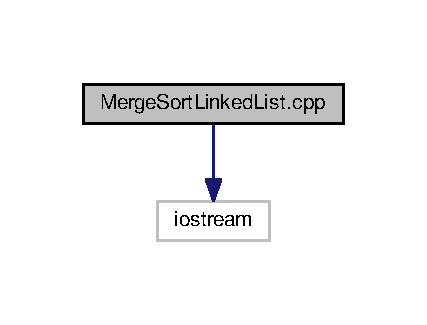
\includegraphics[width=205pt]{MergeSortLinkedList_8cpp__incl}
\end{center}
\end{figure}
\subsection*{Classes}
\begin{DoxyCompactItemize}
\item 
struct \hyperlink{structnode}{node}
\end{DoxyCompactItemize}
\subsection*{Functions}
\begin{DoxyCompactItemize}
\item 
\hyperlink{structnode}{node} $\ast$ \hyperlink{MergeSortLinkedList_8cpp_a587f3ecc3187b212f1e1c757638271cb}{New\+Node} (int d)
\item 
\hyperlink{structnode}{node} $\ast$ \hyperlink{MergeSortLinkedList_8cpp_ae40684a865c3a49ffe398571a7991482}{Add\+To\+List} (\hyperlink{structnode}{node} $\ast$tail, int data)
\item 
\hyperlink{structnode}{node} $\ast$ \hyperlink{MergeSortLinkedList_8cpp_ac668b542d448c2016db19bb65d3910a6}{Merge} (\hyperlink{structnode}{node} $\ast$h1, \hyperlink{structnode}{node} $\ast$h2)
\item 
void \hyperlink{MergeSortLinkedList_8cpp_afe97025c3170e7a45b91e7afeeeb8646}{Merge\+Sort} (\hyperlink{structnode}{node} $\ast$$\ast$head)
\item 
int \hyperlink{MergeSortLinkedList_8cpp_ae66f6b31b5ad750f1fe042a706a4e3d4}{main} ()
\end{DoxyCompactItemize}


\subsection{Function Documentation}
\index{Merge\+Sort\+Linked\+List.\+cpp@{Merge\+Sort\+Linked\+List.\+cpp}!Add\+To\+List@{Add\+To\+List}}
\index{Add\+To\+List@{Add\+To\+List}!Merge\+Sort\+Linked\+List.\+cpp@{Merge\+Sort\+Linked\+List.\+cpp}}
\subsubsection[{\texorpdfstring{Add\+To\+List(node $\ast$tail, int data)}{AddToList(node *tail, int data)}}]{\setlength{\rightskip}{0pt plus 5cm}{\bf node}$\ast$ Add\+To\+List (
\begin{DoxyParamCaption}
\item[{{\bf node} $\ast$}]{tail, }
\item[{int}]{data}
\end{DoxyParamCaption}
)}\hypertarget{MergeSortLinkedList_8cpp_ae40684a865c3a49ffe398571a7991482}{}\label{MergeSortLinkedList_8cpp_ae40684a865c3a49ffe398571a7991482}

\begin{DoxyCode}
24 \{
25     \textcolor{keyword}{struct }\hyperlink{structnode}{node} *newnode;
26     newnode = \hyperlink{MergeSortLinkedList_8cpp_a587f3ecc3187b212f1e1c757638271cb}{NewNode}(\hyperlink{structnode_a2d890bb9f6af0ffd73fe79b21124c2a2}{data});
27  
28     \textcolor{keywordflow}{if}(tail == NULL)
29     \{
30         tail = newnode;
31     \}
32     \textcolor{comment}{// If tail is not null assign newnode to the next of tail.}
33     \textcolor{keywordflow}{else}
34     \{
35         tail->\hyperlink{structnode_aad210fa7c160a49f6b9a3ffee592a2bc}{next} = newnode;
36         \textcolor{comment}{// Shift tail pointer to the added node.}
37         tail = tail->\hyperlink{structnode_aad210fa7c160a49f6b9a3ffee592a2bc}{next};
38     \}
39  
40     \textcolor{keywordflow}{return} tail;
41 \}
\end{DoxyCode}


Here is the call graph for this function\+:
\nopagebreak
\begin{figure}[H]
\begin{center}
\leavevmode
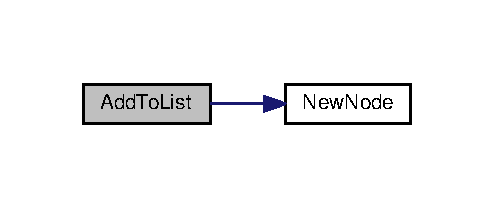
\includegraphics[width=237pt]{MergeSortLinkedList_8cpp_ae40684a865c3a49ffe398571a7991482_cgraph}
\end{center}
\end{figure}


\index{Merge\+Sort\+Linked\+List.\+cpp@{Merge\+Sort\+Linked\+List.\+cpp}!main@{main}}
\index{main@{main}!Merge\+Sort\+Linked\+List.\+cpp@{Merge\+Sort\+Linked\+List.\+cpp}}
\subsubsection[{\texorpdfstring{main()}{main()}}]{\setlength{\rightskip}{0pt plus 5cm}int main (
\begin{DoxyParamCaption}
{}
\end{DoxyParamCaption}
)}\hypertarget{MergeSortLinkedList_8cpp_ae66f6b31b5ad750f1fe042a706a4e3d4}{}\label{MergeSortLinkedList_8cpp_ae66f6b31b5ad750f1fe042a706a4e3d4}

\begin{DoxyCode}
145 \{
146     \textcolor{keywordtype}{int} n, i, num;
147     \textcolor{keyword}{struct }\hyperlink{structnode}{node} *head = \textcolor{keyword}{new} \hyperlink{structnode}{node};
148     \textcolor{keyword}{struct }\hyperlink{structnode}{node} *tail = \textcolor{keyword}{new} \hyperlink{structnode}{node};
149     head = NULL;
150     tail = NULL;
151     cout<<\textcolor{stringliteral}{"\(\backslash\)nEnter the number of data element to be sorted: "};
152     cin>>n;
153  
154  
155     \textcolor{comment}{// Create linked list.}
156     \textcolor{keywordflow}{for}(i = 0; i < n; i++)
157     \{
158         cout<<\textcolor{stringliteral}{"Enter element "}<<i+1<<\textcolor{stringliteral}{": "};
159         cin>>num;
160  
161         tail = \hyperlink{MergeSortLinkedList_8cpp_ae40684a865c3a49ffe398571a7991482}{AddToList}(tail, num);
162         \textcolor{keywordflow}{if}(head == NULL)
163             head = tail;
164     \}
165  
166     \textcolor{comment}{// Send reference of head into MergeSort().}
167     \hyperlink{MergeSortLinkedList_8cpp_afe97025c3170e7a45b91e7afeeeb8646}{MergeSort}(&head);
168  
169     \textcolor{comment}{// Printing the sorted data.}
170     cout<<\textcolor{stringliteral}{"\(\backslash\)nSorted Data "};
171  
172     \textcolor{keywordflow}{while}(head != NULL) 
173     \{
174         cout<<\textcolor{stringliteral}{".."}<<head->\hyperlink{structnode_a2d890bb9f6af0ffd73fe79b21124c2a2}{data};
175         head=head->\hyperlink{structnode_aad210fa7c160a49f6b9a3ffee592a2bc}{next};
176     \}
177     \textcolor{keywordflow}{return} 0;   
178 \}\end{DoxyCode}


Here is the call graph for this function\+:
\nopagebreak
\begin{figure}[H]
\begin{center}
\leavevmode
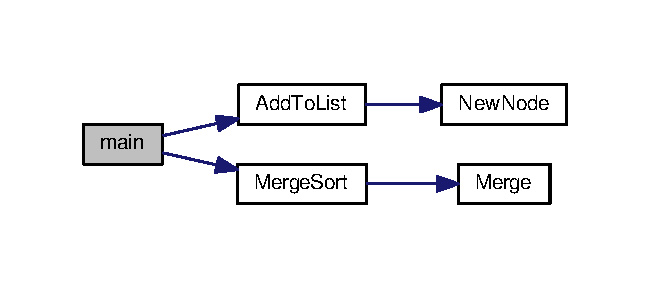
\includegraphics[width=312pt]{MergeSortLinkedList_8cpp_ae66f6b31b5ad750f1fe042a706a4e3d4_cgraph}
\end{center}
\end{figure}


\index{Merge\+Sort\+Linked\+List.\+cpp@{Merge\+Sort\+Linked\+List.\+cpp}!Merge@{Merge}}
\index{Merge@{Merge}!Merge\+Sort\+Linked\+List.\+cpp@{Merge\+Sort\+Linked\+List.\+cpp}}
\subsubsection[{\texorpdfstring{Merge(node $\ast$h1, node $\ast$h2)}{Merge(node *h1, node *h2)}}]{\setlength{\rightskip}{0pt plus 5cm}{\bf node}$\ast$ Merge (
\begin{DoxyParamCaption}
\item[{{\bf node} $\ast$}]{h1, }
\item[{{\bf node} $\ast$}]{h2}
\end{DoxyParamCaption}
)}\hypertarget{MergeSortLinkedList_8cpp_ac668b542d448c2016db19bb65d3910a6}{}\label{MergeSortLinkedList_8cpp_ac668b542d448c2016db19bb65d3910a6}

\begin{DoxyCode}
44 \{
45     \hyperlink{structnode}{node} *t1 = \textcolor{keyword}{new} \hyperlink{structnode}{node};
46     \hyperlink{structnode}{node} *t2 = \textcolor{keyword}{new} \hyperlink{structnode}{node};
47     \hyperlink{structnode}{node} *temp = \textcolor{keyword}{new} \hyperlink{structnode}{node};
48  
49     \textcolor{comment}{// Return if the first list is empty.}
50     \textcolor{keywordflow}{if}(h1 == NULL)
51         \textcolor{keywordflow}{return} h2;
52  
53     \textcolor{comment}{// Return if the Second list is empty.}
54     \textcolor{keywordflow}{if}(h2 == NULL)
55         \textcolor{keywordflow}{return} h1;
56  
57     t1 = h1;
58  
59     \textcolor{comment}{// A loop to traverse the second list, to merge the nodes to h1 in sorted way.}
60     \textcolor{keywordflow}{while} (h2 != NULL)
61     \{
62         \textcolor{comment}{// Taking head node of second list as t2.}
63         t2 = h2;
64  
65         \textcolor{comment}{// Shifting second list head to the next.}
66         h2 = h2->\hyperlink{structnode_aad210fa7c160a49f6b9a3ffee592a2bc}{next};
67         t2->\hyperlink{structnode_aad210fa7c160a49f6b9a3ffee592a2bc}{next} = NULL;
68  
69         \textcolor{comment}{// If the data value is lesser than the head of first list add that node at the beginning.}
70         \textcolor{keywordflow}{if}(h1->\hyperlink{structnode_a2d890bb9f6af0ffd73fe79b21124c2a2}{data} > t2->\hyperlink{structnode_a2d890bb9f6af0ffd73fe79b21124c2a2}{data})
71         \{
72             t2->\hyperlink{structnode_aad210fa7c160a49f6b9a3ffee592a2bc}{next} = h1;
73             h1 = t2;
74             t1 = h1;
75             \textcolor{keywordflow}{continue};
76         \}
77  
78         \textcolor{comment}{// Traverse the first list.}
79         flag:
80         \textcolor{keywordflow}{if}(t1->\hyperlink{structnode_aad210fa7c160a49f6b9a3ffee592a2bc}{next} == NULL)
81         \{
82             t1->\hyperlink{structnode_aad210fa7c160a49f6b9a3ffee592a2bc}{next} = t2;
83             t1 = t1->\hyperlink{structnode_aad210fa7c160a49f6b9a3ffee592a2bc}{next};
84         \}
85         \textcolor{comment}{// Traverse first list until t2->data more than node's data.}
86         \textcolor{keywordflow}{else} \textcolor{keywordflow}{if}((t1->\hyperlink{structnode_aad210fa7c160a49f6b9a3ffee592a2bc}{next})->data <= t2->\hyperlink{structnode_a2d890bb9f6af0ffd73fe79b21124c2a2}{data})
87         \{
88             t1 = t1->\hyperlink{structnode_aad210fa7c160a49f6b9a3ffee592a2bc}{next};
89             \textcolor{keywordflow}{goto} flag;
90         \}
91         \textcolor{keywordflow}{else}
92         \{
93             \textcolor{comment}{// Insert the node as t2->data is lesser than the next node.}
94             temp = t1->\hyperlink{structnode_aad210fa7c160a49f6b9a3ffee592a2bc}{next};
95             t1->\hyperlink{structnode_aad210fa7c160a49f6b9a3ffee592a2bc}{next} = t2;
96             t2->\hyperlink{structnode_aad210fa7c160a49f6b9a3ffee592a2bc}{next} = temp;
97         \}
98     \}
99  
100     \textcolor{comment}{// Return the head of new sorted list.}
101     \textcolor{keywordflow}{return} h1;
102 \}
\end{DoxyCode}
\index{Merge\+Sort\+Linked\+List.\+cpp@{Merge\+Sort\+Linked\+List.\+cpp}!Merge\+Sort@{Merge\+Sort}}
\index{Merge\+Sort@{Merge\+Sort}!Merge\+Sort\+Linked\+List.\+cpp@{Merge\+Sort\+Linked\+List.\+cpp}}
\subsubsection[{\texorpdfstring{Merge\+Sort(node $\ast$$\ast$head)}{MergeSort(node **head)}}]{\setlength{\rightskip}{0pt plus 5cm}void Merge\+Sort (
\begin{DoxyParamCaption}
\item[{{\bf node} $\ast$$\ast$}]{head}
\end{DoxyParamCaption}
)}\hypertarget{MergeSortLinkedList_8cpp_afe97025c3170e7a45b91e7afeeeb8646}{}\label{MergeSortLinkedList_8cpp_afe97025c3170e7a45b91e7afeeeb8646}

\begin{DoxyCode}
107 \{
108     \hyperlink{structnode}{node} *first = \textcolor{keyword}{new} \hyperlink{structnode}{node};
109     \hyperlink{structnode}{node} *second = \textcolor{keyword}{new} \hyperlink{structnode}{node};
110     \hyperlink{structnode}{node} *temp = \textcolor{keyword}{new} \hyperlink{structnode}{node};
111     first = *head;
112     temp = *head;
113  
114     \textcolor{comment}{// Return if list have less than two nodes.}
115     \textcolor{keywordflow}{if}(first == NULL || first->\hyperlink{structnode_aad210fa7c160a49f6b9a3ffee592a2bc}{next} == NULL)
116     \{
117         \textcolor{keywordflow}{return};
118     \}
119     \textcolor{keywordflow}{else}
120     \{
121         \textcolor{comment}{// Break the list into two half as first and second as head of list.}
122         \textcolor{keywordflow}{while}(first->\hyperlink{structnode_aad210fa7c160a49f6b9a3ffee592a2bc}{next} != NULL)
123         \{
124             first = first->\hyperlink{structnode_aad210fa7c160a49f6b9a3ffee592a2bc}{next};
125             \textcolor{keywordflow}{if}(first->\hyperlink{structnode_aad210fa7c160a49f6b9a3ffee592a2bc}{next} != NULL)
126             \{
127                 temp = temp->\hyperlink{structnode_aad210fa7c160a49f6b9a3ffee592a2bc}{next};
128                 first = first->\hyperlink{structnode_aad210fa7c160a49f6b9a3ffee592a2bc}{next};
129             \}
130         \}
131         second = temp->\hyperlink{structnode_aad210fa7c160a49f6b9a3ffee592a2bc}{next};
132         temp->\hyperlink{structnode_aad210fa7c160a49f6b9a3ffee592a2bc}{next} = NULL;
133         first = *head;
134     \}
135  
136     \textcolor{comment}{// Implementing divide and conquer approach.}
137     \hyperlink{MergeSortLinkedList_8cpp_afe97025c3170e7a45b91e7afeeeb8646}{MergeSort}(&first);
138     \hyperlink{MergeSortLinkedList_8cpp_afe97025c3170e7a45b91e7afeeeb8646}{MergeSort}(&second);
139  
140     \textcolor{comment}{// Merge the two part of the list into a sorted one.      }
141     *head = \hyperlink{MergeSortLinkedList_8cpp_ac668b542d448c2016db19bb65d3910a6}{Merge}(first, second);
142 \}
\end{DoxyCode}


Here is the call graph for this function\+:
\nopagebreak
\begin{figure}[H]
\begin{center}
\leavevmode
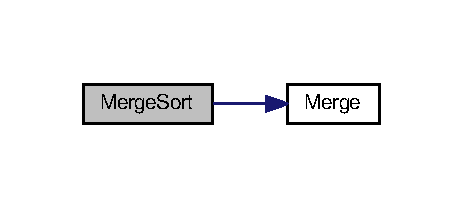
\includegraphics[width=222pt]{MergeSortLinkedList_8cpp_afe97025c3170e7a45b91e7afeeeb8646_cgraph}
\end{center}
\end{figure}


\index{Merge\+Sort\+Linked\+List.\+cpp@{Merge\+Sort\+Linked\+List.\+cpp}!New\+Node@{New\+Node}}
\index{New\+Node@{New\+Node}!Merge\+Sort\+Linked\+List.\+cpp@{Merge\+Sort\+Linked\+List.\+cpp}}
\subsubsection[{\texorpdfstring{New\+Node(int d)}{NewNode(int d)}}]{\setlength{\rightskip}{0pt plus 5cm}{\bf node}$\ast$ New\+Node (
\begin{DoxyParamCaption}
\item[{int}]{d}
\end{DoxyParamCaption}
)}\hypertarget{MergeSortLinkedList_8cpp_a587f3ecc3187b212f1e1c757638271cb}{}\label{MergeSortLinkedList_8cpp_a587f3ecc3187b212f1e1c757638271cb}

\begin{DoxyCode}
14 \{
15     \textcolor{keyword}{struct }\hyperlink{structnode}{node} *temp = \textcolor{keyword}{new} \hyperlink{structnode}{node};
16     temp->\hyperlink{structnode_a2d890bb9f6af0ffd73fe79b21124c2a2}{data} = d;
17     temp->\hyperlink{structnode_aad210fa7c160a49f6b9a3ffee592a2bc}{next} = NULL;
18     \textcolor{comment}{// Returning temp as the new node.}
19     \textcolor{keywordflow}{return} temp;
20 \}
\end{DoxyCode}

%--- End generated contents ---

% Index
\backmatter
\newpage
\phantomsection
\clearemptydoublepage
\addcontentsline{toc}{chapter}{Index}
\printindex

\end{document}
